\documentclass[10pt,a4paper]{article}
\usepackage[utf8]{inputenc}
\usepackage{
	polski,
	pdflscape,
	graphicx,
	multirow,
	longtable,
	array,
	enumitem,
	listings,
	everypage,
	geometry,
	color,
	makecell,
	float
}

\definecolor{codegreen}{rgb}{0,0.6,0}
\definecolor{codegray}{rgb}{0.5,0.5,0.5}
\definecolor{codepurple}{rgb}{0.58,0,0.82}
\definecolor{backcolour}{rgb}{0.95,0.95,0.92}

\lstdefinestyle{mystyle}{
    backgroundcolor=\color{backcolour},   
    commentstyle=\color{codegreen},
    keywordstyle=\color{magenta},
    numberstyle=\tiny\color{codegray},
    stringstyle=\color{codepurple},
    basicstyle=\footnotesize,
    breakatwhitespace=false,         
    breaklines=true,                 
    captionpos=b,                    
    keepspaces=true,                 
    numbers=left,                    
    numbersep=5pt,                  
    showspaces=false,                
    showstringspaces=false,
    showtabs=false,                  
    tabsize=2
}
 
\lstset{style=mystyle}

\geometry{ 
	top=20mm,
	bottom=30mm
}

\renewcommand\labelenumii{\arabic{enumii}.}

\renewcommand\theadfont{\bfseries}

\newcommand{\Lpagenumber}{\ifdim\textwidth=\linewidth\else\bgroup
  \dimendef\margin=0
  \ifodd\value{page}\margin=\oddsidemargin
  \else\margin=\evensidemargin
  \fi
  \raisebox{\dimexpr -\topmargin-\headheight-\headsep-0.5\linewidth}[0pt][0pt]{%
    \rlap{\hspace{\dimexpr \margin+\textheight+\footskip}%
    \llap{\rotatebox{90}{\thepage}}}}%
\egroup\fi}
\AddEverypageHook{\Lpagenumber}%

\lstset{language=SQL,
	basicstyle=\ttfamily\scriptsize,
    keywordstyle=\color{blue}\ttfamily,
    stringstyle=\color{red}\ttfamily,
    commentstyle=\color{green}\ttfamily,
    breaklines=true
}

\author{
  \small Mateusz Forc\\
  \small Wiktor Franus\\
  \small Hubert Jatkowski\\
  \small Przemysław Kopański\\
  \small Grzegorz Staniszewski\\
}
\title{Sklep Internetowy}
\begin{document}
  \maketitle
  \begin{abstract}
    \begin{center}
    Aplikacja bazodanowa realizowana na przedmiot Bazy Danych 2 w semestrze 2016Z.
    \end{center}
  \end{abstract}
  \tableofcontents
  \newpage
  \begin{landscape}
  \pagestyle{empty}
  \section{Projekt Bazy Danych}
  
    \subsection{Diagram ER wraz z opisem związków}
      \begin{center}
        \includegraphics[scale=0.4]{ER}
      \end{center}
   \end{landscape}
    
    \newpage 
    \subsection{Opis Encji}
     \textbf{Client} - encja reprezentująca klienta
      \begin{center}
        \begin{tabular}{| m{3cm} | m{3cm} | m{3cm} | m{3cm} |}
          \hline
          Nazwa atrybutu & Typ danych & Obligatoryjność & Opis\\ \hline
		  id        & PK INTEGER    & NOT NULL 		    & -\\ \hline
		  name      & STRING        & NOT NULL 			& -\\ \hline
		  surname   & STRING        & NOT NULL 			& -\\ \hline
		  birthdate & DATE          & NOT NULL 			& -\\ \hline
		  address   & TEXT          & NOT NULL 			& -\\ \hline
		  email     & UNIQUE STRING & NOT NULL 			& -\\ \hline
		  login     & UNIQUE STRING & NOT NULL 			& -\\ \hline
		  password  & STRING        & NOT NULL 			& -\\ \hline
		\end{tabular}
	  \end{center}

	  \flushleft \textbf{Employee} - encja reprezentująca pracownika
	  \begin{center}
        \begin{tabular}{| m{3cm} | m{3cm} | m{3cm} | m{3cm} |}
          \hline
          Nazwa atrybutu & Typ danych 	 & Obligatoryjność & Opis\\ \hline
		  id  			 & PK INTEGER 	 & NOT NULL 	   & -\\ \hline
		  name 			 & STRING 	  	 & NOT NULL 	   & -\\ \hline
		  surname 		 & STRING 	  	 & NOT NULL 	   & -\\ \hline
		  pesel 		 & UNIQUE STRING & NOT NULL 	   & -\\ \hline
		  birthdate 	 & DATE 		 & NOT NULL 	   & -\\ \hline
		  address 	  	 & TEXT 		 & NOT NULL 	   & -\\ \hline
		  email 		 & UNIQUE STRING & NOT NULL 	   & -\\ \hline
		  login 		 & UNIQUE STRING & NOT NULL 	   & -\\ \hline
		  password 		 & STRING 		 & NOT NULL 	   & -\\ \hline
		\end{tabular}
	  \end{center}
	  
	  \flushleft \textbf{Review} - encja reprezentująca opinię klienta o towarze
	  \begin{center}
        \begin{tabular}{| m{3cm} | m{3cm} | m{3cm} | m{3cm} |}
          \hline
          Nazwa atrybutu & Typ danych & Obligatoryjność & Opis\\ \hline
		  id 			 & PK INTEGER & NOT NULL 	    & -\\ \hline
		  rating 		 & INTEGER 	  & NOT NULL 		& Ocena produktu w skali od 1 do 5\\ \hline
		  comment 		 & TEXT 	  & NOT NULL 		& Tekst opinii wprowadzony przez autora\\ \hline
		  date 			 & TIMESTAMP  & NOT NULL 		& Data dodania opinii\\ \hline
		  client\_id 	 & FK INTEGER & NOT NULL 		& ID klienta, który dodał opinię\\ \hline
		  item\_id 		 & FK INTEGER & NOT NULL 		& ID produktu, którego dotyczy opinia\\ \hline
		\end{tabular}
	  \end{center}
	
	  %\newpage
	  \flushleft \textbf{Order} - encja reprezentująca zamówienie na towary
      \begin{center}
        \begin{tabular}{| m{3cm} | m{3cm} | m{3cm} | m{3cm} |}
          \hline
          Nazwa atrybutu 	   & Typ danych & Obligatoryjność & Opis\\ \hline
		  id 		  	 	   & PK INTEGER & NOT NULL 		  & -\\ \hline
		  date 			 	   & TIMESTAMP  & NOT NULL 		  & Data złożenia zamówienia\\ \hline
		  status 		 	   & INTEGER 	& NOT NULL 		  & Informacja, czy zamówienie jest złożone, 
		  												        w realizacji, czy sfinalizowane\\ \hline
		  status\_change\_date & TIMESTAMP 	& NOT NULL 		  & Data ostatniej zmiany statusu\\ \hline
		  payment\_status 	   & INTEGER 	& NOT NULL 		  & Status płatności za zamówienie\\ \hline
		  client\_id 		   & FK INTEGER & NOT NULL 		  & ID klienta, który złożył zamówienie\\ \hline
		\end{tabular}
	  \end{center}

	  \newpage
	  \flushleft \textbf{Item} - encja reprezentująca towar na składzie
      \begin{center}
        \begin{tabular}{| m{3cm} | m{3cm} | m{3cm} |  m{3cm} |}
          \hline
          Nazwa atrybutu & Typ danych & Obligatoryjność & Opis\\ \hline
		  id 			 & PK INTEGER & NOT NULL 		& -\\ \hline
		  name 			 & STRING 	  & NOT NULL 		& Nazwa towaru\\ \hline
		  price 		 & DECIMAL 	  & NOT NULL 		& Cena towaru\\ \hline
		  description 	 & STRING 	  & NOT NULL 		& Dokładniejszy opis towaru\\ \hline
		  in\_stock 	 & INTEGER 	  & NOT NULL 		& Liczba sztuk towaru na składzie\\ \hline
		  category\_id 	 & FK INTEGER & NOT NULL 		& ID kategorii, do której należy towar\\ \hline
		\end{tabular}
	  \end{center}

	  \flushleft \textbf{Order\_Item} - encja pośrednicząca pomiędzy Order i Item
	  \begin{center}
        \begin{tabular}{| m{3cm} | m{3cm} | m{3cm} |  m{3cm} |}
          \hline
          Nazwa atrybutu & Typ danych & Obligatoryjność & Opis\\ \hline
		  id 			 & PK INTEGER & NOT NULL 		& -\\ \hline
		  quantity 	 	 & INTEGER 	  & NOT NULL 		& Liczba sztuk towaru w zamówieniu\\ \hline
		  price 		 & DECIMAL 	  & NOT NULL 		& Cena towaru za sztukę, 
		  							               		  za który został sprzedany w danym zamówieniu\\ \hline
		  order\_id 	 & FK INTEGER & NOT NULL 		& ID zamówienia, do którego należy pozycja\\ \hline
		  item\_id 		 & FK INTEGER & NOT NULL 		& ID towaru, na który wskazuje pozycja\\ \hline
		\end{tabular}
	  \end{center}
	   
	  %\newpage
	  \flushleft \textbf{Category} - encja reprezentująca kategorię, do której może należeć towar
      \begin{center}
        \begin{tabular}{| m{3cm} | m{3cm} | m{3cm} |  m{3cm} |}
          \hline
          Nazwa atrybutu & Typ danych & Obligatoryjność & Opis\\ \hline
		  id 			 & PK INTEGER & NOT NULL 		& -\\ \hline
		  name 			 & STRING 	  & NOT NULL 		& Nazwa kategorii\\ \hline
		\end{tabular}
	  \end{center}

	  \flushleft \textbf{Invoice} - encja reprezentująca fakturę
	  \begin{center}
        \begin{tabular}{| m{3cm} | m{3cm} | m{3cm} |  m{3cm} |}
          \hline
          Nazwa atrybutu & Typ danych 	  & Obligatoryjność & Opis\\ \hline
          order\_id 	 & PK FK INTEGER  & NOT NULL 		& ID zamówienia, na które została wystawiona faktura\\ \hline
		  unique\_no 	 & UNIQUE INTEGER & NOT NULL 		& Numer faktury\\ \hline
		\end{tabular}
	  \end{center}
  	\newpage

    \subsection{Słownik pojęć}
        \begin{itemize}
		  \item \textbf{Sklep internetowy} – aplikacja, która jest przedmiotem niniejszego projektu.
		  \item \textbf{Administrator sklepu} - pracownik sklepu zarządzający kontami innych pracowników
          \item \textbf{Klient/Użytkownik anonimowy} – osoba niezarejestrowana w systemie,
           	    		korzystająca z serwisu w celu zakupu towarów.
		  \item \textbf{Klient/Użytkownik zarejestrowany} – osoba zarejestrowana w systemie (posiadająca konto),
		  				korzystająca z serwisu w celu zakupu towarów.
		  \item \textbf{Pracownik sklepu} – użytkownik zarejestrowany zarządzający aplikacją, posiada dostęp do edycji 									towarów, kategorii, zamówień i opinii w sklepie internetowym.
		  \item \textbf{Nazwa użytkownika} – nazwa, którą użytkownik będzie posługiwał i identyfikował się w serwisie,
		  	    		nazwa użytkownika jest niezbędna podczas logowania.
		  \item \textbf{Hasło użytkownika} – ciąg znaków, używany do logowania się do serwisu oraz uzyskiwania dostępu 
		  				do pełnych funkcji serwisu.
		  \item \textbf{Towar} – produkt sprzedawany.
		  \item \textbf{Zamówienie} – lista towarów (wraz z ilością sztuk) wybranych i zatwierdzonych przez 
		  				klienta w celu zakupu.
		  \item \textbf{Opinia} - komentarz słowny i/lub ocena punktowa w skali 1-5 użytkownika zarejestrowanego 
		  				na temat zakupionego towaru
		  \item \textbf{Koszyk} – podręczna lista towarów wybranych przez klienta.
		  \item \textbf{E-faktura VAT} – dokument elektroniczny wystawiany przez czynnych podatników VAT, 
		  				potwierdzający przeprowadzenie czynności podlegającej opodatkowaniu VAT
		  \item \textbf{Przeglądarka internetowa} – program komputerowy służący do pobierania i 
		  	    		wyświetlania stron internetowych udostępnianych przez serwery WWW.
		\end{itemize}
		
	  \newpage
	  \subsection{Wymagania Funkcjonalne}
	  	\flushleft
          \begin{longtable}{| m{0.5cm} | m{4cm} | p{6cm} | m{1.5cm} |}
            \hline
            Lp. & Nazwa wymagania 						& Opis 										& Priorytet\\ \hline
            \multicolumn{4}{|l|}{Funkcjonalności dostępne bez konieczności logowania}\\ \hline
            1.  & Wyświetlenie listy dostępnych towarów & Wyświetlenie listy zawierającej zdjęcie, 
            											  nazwę i cenę dla każdego towaru.			& 1\\ \hline
            2.  & Wyświetlanie szczegółowych danych na 
            	  temat konkretnego towaru				& Wyświetlanie widoku szczegółowego 
            	  										  zawierającego nazwę, zdjęcie, opis oraz
            	  										  cenę konkretnego towaru.					& 1\\ \hline
			3.  & Wyszukiwanie towarów					& Wyszukiwanie i wyświetlanie listy 
														  towarów o wpisanej nazwie. Powinny zostać 
														  wyświetlone zarówno towary, których nazwa 
														  jest identyczna z wpisaną, jak i te,
														  których nazwa częściowo pokrywa się 
														  ze wpisaną frazą.							& 2\\ \hline
			4.	& Rejestracja nowego klienta w systemie & Rejestracja nowego użytkownika w systemie
														  wymaga podania danych obowiązkowych, tj.:
														  
														  \begin{itemize}[label={--}]
														  \item Imię i nazwisko użytkownika
														  \item Adres e-mail użytkownika
														  \item Nazwa użytkownika
														  \item Hasło użytkownika
														  \item Adres zamieszkania użytkownika
														  \end{itemize}
														  Oraz danych opcjonalnych, tj.:
														  \begin{itemize}[label={--}]
														  \item Adres do wysyłki
														      (jeżeli inny niż adres zamieszkania)
														  \item Datę urodzenia użytkownika.
														  \end{itemize}								& 1\\ \hline
			5. & Logowanie klienta						& Uwierzytelnianie użytkownika za pomocą 
														  nazwy użytkownika i hasła. 
														  Zawartość koszyka nie ulega zmianie 
														  po zalogowaniu.							& 1\\ \hline
														  
			6. & Wyświetlanie informacji 
			     o przedsiębiorstwie prowadzącym 
			     niniejszy sklep internetowy			& Wyświetlanie nazwy, pełnego adresu 
			     										  oraz numeru telefonu przedsiębiorstwa.    & 3\\ \hline
			\multicolumn{4}{|c|}{Funkcjonalności dostępne dla zarejestrowanego użytkownika
			wszystkie powyższe oraz:}\\ \hline
			7. & Edytowanie swoich danych				& Możliwość edycji poniższych danych:
														  \begin{itemize}[label={--}]
														  \item Adresu e-mail użytkownika
														  \item Hasła użytkownika
														  \item Adresu zamieszkania użytkownika
														  \item Adresu do wysyłki.					
														  \end{itemize}								& 2\\ \hline
										  
			8. & Dodawanie towarów do koszyka 			& Dodawanie do koszyka towaru wybranego 
														  przez użytkownika. Ponowne dodanie tego
														  samego towaru do koszyka skutkuje 
														  zwiększeniem ilości sztuk 
														  tego towaru w koszyku.					& 1\\ \hline
														  
			9. & Zmiana ilości sztuk towarów w koszyku & Zmiana ilości sztuk dla wybranego towaru 
														 znajdującego się aktualnie w koszyku. 		& 2\\ \hline
														 
			10.& Usuwanie towarów z koszyka			   & Usuwanie z koszyka towarów wybranych 
														 przez użytkownika. 						& 1\\ \hline
			11.& Składanie zamówienia				   & Składanie zamówienia na towar znajdujący
														 się aktualnie w koszyku. Po złożeniu 
														 zamówienia wyświetlane jest jego 
														 potwierdzenie. Potwierdzenie to jest 
														 również wysyłane na adres e-mail
														 użytkownika, który to zamówienie złożył.   & 1\\ \hline
			12.& Śledzenie statusu zamówienia		   & Wyświetlanie poprzednich oraz aktualnego
														 statusu zamówienia. Wyświetlanie 
														 daty i godziny każdej zmiany statusu. 
														 Zamówienie może mieć w danym momencie 
														 jeden z następujących statusów:
														 \begin{itemize}[label={--}]
														 \item zarejestrowane
														 \item w realizacji
														 \item wysłane
														 \item zrealizowane
														 \item anulowane
														 \end{itemize}								& 2\\ \hline
			13.& Wyświetlanie historii zamówień        & Wyświetlanie chronologicznej listy wszystkich
			 											 zamówień złożonych przez 
			 											 zalogowanego użytkownika						& 1\\ \hline
			 											 
			14.& Zlecenie wystawienia e-faktury VAT    & Możliwość zlecenia wystawienia e-faktury VAT 
														 w momencie składania zamówienia				& 2\\ \hline
			15.& Dodawanie opinii na temat towaru	   & Dodawanie opinii o wybranym produkcie poprzez 
														 napisanie komentarza oraz/lub wybranie 
														 ilości „gwiazdek” w skali 1-5,
														 gdzie 5 oznacza wartość najlepszą.				& 3\\ \hline
			 \multicolumn{4}{|c|}{Funkcjonalności dostępne dla pracownika sklepu
			 					  wszystkie powyższe oraz:}\\ \hline
			16.& Dodawanie towaru					   & Dodawanie nowego towaru do bazy dostępnych
			 											 towarów poprzez podanie jego: nazwy,
			 											 kategorii do której należy, opisu,
			 											 ceny oraz ilości sztuk. 
			 											 Do każdego towaru można dodać zdjęcie. 
			 											 W przypadku nie dodania zdjęcia przez pracownika
			 											 sklepu, system dodaje zdjęcie domyślne.		& 1\\ \hline
			17.& Usuwanie towaru					   & Usuwanie wybranego towaru z bazy.				& 1\\ \hline
			18.& Edytowanie danych towaru			   & Możliwość edycji wszystkich danych powiązanych
														 z wybranym towarem.							& 1\\ \hline
			19.& Dodawanie kategorii				   & Dodawanie kategorii towarów poprzez 
														 podanie jej nazwy i opisu.						& 1\\ \hline
			20.& Usuwanie kategorii					   & Usuwanie wybranej kategorii z bazy.			& 1\\ \hline
			21.& Zmiana statusu zamówienia			   & Zmiana statusu zamówienia na inny. 
														 Dostępne statusy wymieniono w punkcie 12.		& 2\\ \hline
			22.&Usuwanie opinii 					   & Usuwanie z bazy danych opinii wystawionych
														 przez użytkowników								& 3\\ \hline
														 
			\multicolumn{4}{|c|}{Funkcjonalności dostępne dla administratora sklepu}\\ \hline
			23.&Dodawanie pracownika				   & Dodawanie nowego konta pracownika do systemu.
														 Dodanie pracownika wymaga podania identycznych
														 danych jak przy rejestracji klienta
														 z uwzględnieniem poniższych wyjątków:
														 \begin{itemize}[label={--}]
														 \item Data urodzenia jest obowiązkowa
														 \item Wymagane jest również podanie numeru PESEL.  
														 \end{itemize}									& 1\\ \hline
			24.&Usuwanie pracownika					   & Usuwanie wybranego użytkownika z bazy.			& 1\\ \hline
			25.&Edytowanie danych pracownika		   & Możliwość edycji wszystkich danych 
														 wybranego użytkownika.							& 1\\ \hline
     		\multicolumn{4}{|c|}{Pozostałe funkcjonalności}\\ \hline
			26.&Generowanie e-faktur VAT			   & Generowanie e-faktur VAT za zamówienia,
														 dla których zostały wysłane zlecenia 
														 wystawienia e-faktury VAT						& 2\\ \hline
			27.&Wysyłanie e-faktur do klienta
			    zarejestrowanego					   & Wysyłanie wygenerowanych e-faktur na 
			    										 adres e-mail klienta, który złożył 
			    										 zlecenie wygenerowania e-faktury 
			    										 dla konkretnego zamówienia.					& 2\\ \hline


     \end{longtable}
     
     \newpage
     \subsection{Wymagania niefunkcjonalne:}
     \begin{enumerate}
	   \item Dostęp do sklepu internetowego przez 24h na dobę.
	   \item Dostęp do sklepu internetowego za pomocą przeglądarki internetowej.
	   \item W celu złożenia zamówienia konieczna jest rejestracja oraz zalogowanie w systemie.
	   \item Każdy użytkownik ma ograniczone prawa dostępu do systemu.
	   \item Konto każdego użytkownika chronione jest nazwą użytkownika i hasłem. Hasło nie może być przechowywane w bazie 				     danych w formie jawnej. Jest zaszyfrowane funkcją skrótu.
	   \item System powinien obsługiwać około 10 000 towarów.
	   \item System powinien obsługiwać około 100 000 zarejestrowanych użytkowników.
	   \item System powinien obsługiwać około 100 jednocześnie połączonych użytkowników.
	   \item E-faktury VAT generowane przez sklep internetowy muszą spełniać wszystkie wymogi 
		     polskiego prawa dotyczące e-faktur. 
	  \end{enumerate}
	  
	  \begin{landscape}
	  \pagestyle{empty}
      \subsection{Schemat logiczny}
        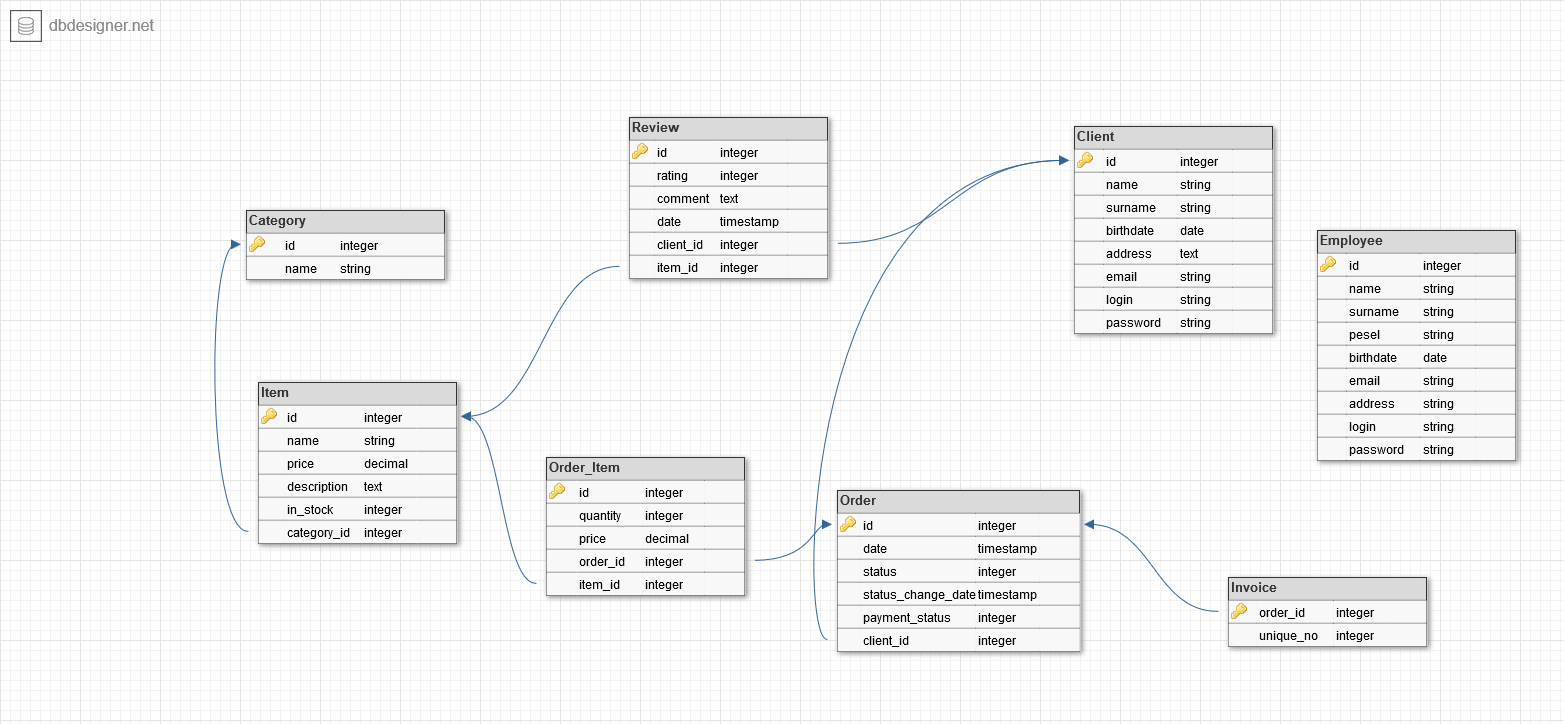
\includegraphics[scale=0.4]{schematlogiczny}
      \end{landscape}
      
      \newpage
      \subsection{Skrypt DDL tworzący bazę danych}
		\lstinputlisting{DDL_schema.sql} 
		
	\newpage
	\section{Projekt Aplikacji}
	  \subsection{ Hierarchia menu}
      \small
	  \begin{itemize}
        
        \item Strona główna - dostępna bez logowania
        \begin{itemize}
          \item Logowanie
		  \item Rejestracja
		  \item Kategorie
		  \begin{itemize}
 		    \item Przeglądaj kategorie
 			  \begin{itemize}
		        \item Wyświetl towary
		      \end{itemize}
		  \item Towary
		  \begin{itemize}
		     \item Przeglądaj towary
		  \end{itemize}
		  \item Wyszukiwarka
		  \item Kontakt
	      \end{itemize}
        \end{itemize}
	    
	    \item Strona pracownika
		\begin{itemize}
		\item Zamówienia
		  \begin{itemize}
		    \item Przeglądaj
		    \begin{itemize}
		    \item Edytuj
		    \end{itemize}
		  \end{itemize}
		\item Towary
		\begin{itemize}
		  \item Przeglądaj towary
		  \begin{itemize}
		    \item Edytuj
			\item Usuń
		  \end{itemize}
		  \item Dodaj
		\end{itemize}
		\item Kategorie
		\begin{itemize}
		  \item Przeglądaj kategorie
		  \begin{itemize}
		    \item Wyświetl towary
			\item Edytuj
			\item Usuń
		  \end{itemize}
		  \item Dodaj
		\end{itemize}
		\item Wyszukiwarka
	    \end{itemize}
		
		\item Strona klienta
		\begin{itemize}
		  \item Moje dane
		  \begin{itemize}
		    \item Edytuj dane
		  \end{itemize}
		  \item Koszyk
		  \begin{itemize}
		    \item Edycja koszyka
		  \end{itemize}
		  \item Moje zamówienia
		  \begin{itemize}
		    \item Zatwierdź zamówienie
		    \item Przeglądaj zamówienia
		    \begin{itemize}
		      \item Szczegóły zamówienia
		    \end{itemize}
		  \end{itemize}		         
		  \item Kategorie
		  \begin{itemize}
		    \item Przeglądaj kategorie
		    \begin{itemize}
		      \item Wyświetl towary
		    \end{itemize}
		  \end{itemize}
		  \item Towary
	        \begin{itemize}
              \item Przeglądaj towary
	          \begin{itemize}
		        \item Dodaj do koszyka
	          \end{itemize}
            \end{itemize}
          \end{itemize}
		       
		  \item Strona administratora
		  \begin{itemize}
		    \item Pracownicy
		    \begin{itemize}
		      \item Przeglądaj
		      \begin{itemize}
		        \item Edytuj
		        \item Usuń
		      \end{itemize}
		        \item Dodaj
		    \end{itemize}
		  \end{itemize}
		\end{itemize}
		
		\subsection{Podział na moduły}
		\begin{itemize}
		  \item Diagram modułów
  		  \includegraphics[scale=0.7]{Modules}
		  \item Aplikacja składa się z czterech modułów
		  \begin{itemize}
   	 	    \item \textbf{Accounts} : Moduł jest odpowiedzialny za zarządzanie kontami użytkowników 
   	 	  	    					: logowanie, rejestracja konta
 		  	\item \textbf{Client}   : Moduł umożliwia klientowi przeglądanie asortymentu oferowanego
 		     						  przez serwis, edycję koszyka, składanie zamówień, 
 		     						  znajduje się tutaj również wyświetlanie strony głównej
		  	\item \textbf{Employee} : Moduł pozwala uprzywilejowanemu użytkownikowi wykonywać operacje
		  							  typowe dla pracownika sklepu, tj. przeglądanie listy zamówień, 
		  							  zmiana ich statusu
		  	\item \textbf{Data
		  			    Access
		  				Object     }: Moduł trzyma w sobie wszystkie tabele poza tabelami użytkowników 
		  							  tzn. klientów i pracowników sklepu umożliwiając zapytania do bazy danych
 		  \end{itemize}
		\end{itemize}
		
		\subsection{Podział realizacji funkcjonalności}
		Klient - strona internetowa z przyjaznym interfejsem.
		\begin{itemize}
		  \item odpowiada za prezentacje graficzną danych dla klienta oraz pracownika
		  \item wyświetla towary, wyświetla szczegółowe informacje o towarze
		  \item umożliwia wyszukiwanie towaru po kategorii i/lub nazwie
		  \item umożliwia zalogowanie i rejestracje
		  \item obsługuje koszyk klienta - umożliwia dodanie/usunięcie produktu do/z koszyka, 
		  		modyfikacja ilości sztuk zamawianego towaru, umożliwia złożenie zamówienia 	
		  \item wyświetla wszystkie złożone przez danego klienta zamówienia wraz z informacjami o nich 
		  		(tj. lista zamówionych towarów, status zamówienia)
		\end{itemize}
	
		Serwer
		\begin{itemize}
		  \item komunikuje się z bazą danych, pośrednicząc między klientem a danymi
			 	na poziomie aplikacyjnym zapewnia integralność danych
		  \item obsługuje uwierzytelnienie klienta oraz pracownika
		\end{itemize}

		\newpage
		\subsection{Określenie sposobu realizacji integralności danych}
	    \flushleft
  		\begin{longtable}{| p{0.5cm} | p{4cm} | p{6cm} | p{2cm} |}
  \hline
  Lp & Problem zapewnienia integralności &           Rozwiązanie                 & Zapewnione przez
  																	               [definicja tabel 
  																	               / programowo]\\ \hline
  1. & Przechowywanie w bazie tylko
       określonych statusów zamówienia   &  Zlecenie zmiany statusu zamówienia
         									kontrolowane jest przez serwer.		 & programowo\\ \hline
  2. & Usunięcie zlecenia powoduje
  	   brak integralności				 &  Zablokowanie możliwości usunięcia
  	   										zamówienia. W takiej sytuacji
  	   										zamówienie otrzymuje 
  	   										status anulowane. 					 & programowo\\ \hline
  	   										
  3. & Ocena produktu zawiera wartość
       liczbową od 1 do 5				 &  Podczas próby dodania nowej opinii,
       										serwer sprawdza poprawność 
       										wprowadzonej oceny.					 & programowo\\ \hline
  4. & Faktura reprezentowana
  	   jest unikalnym numerem			 & Przy wstawianiu nowego wpisu
  	    								   do tabeli Invoice, baza danych 
  	    								   generuje i nadaje unikalny numer PK   & definicja tabeli\\ \hline
  5. & Do zlecenia może zostać
       wygenerowana maksymalnie
       jedna faktura					 & Serwer pozwala na wygenerowanie 
       									   faktury tylko w przypadku 
       									   gdy w tabeli Invoice nie ma 
       									   informacji o fakturze przypisanej
       									   do zamówienia						 & programowo\\ \hline
  6. & Faktura zawiera aktualne
       dane klienta - 
       nawet po edycji danych klienta    & Faktura może zostać wygenerowana
                                           tylko w momencie zatwierdzania
                                           zamówienia i zapisywana jest na
                                           dysku w formacie PDF
                                           przez pracownika.					 & programowo\\ \hline
  7. & Usunięcie produktu z bazy
       może spowodować problemy 
       przy przeglądaniu
       historii zamówień				 & Brak możliwości usunięcia towaru. 
       									   W tabeli Item przechowywana jest 
       									   liczba towarów dostępnych 
       									   na stanie sklepu. Gdy wynosi zero 
       									   to nie ma możliwości 
       									   kupienia produktu. 					 & programowo\\ \hline
  8. & Zmiana ceny produktu powoduje
       brak integralności danych przy
       przeglądaniu historii zamówień.   & W tabeli pośredniczącej Order\_Item
     									   przetrzymywana jest ilość sztuk
     									   danego produktu i cena za sztukę
     									   w momencie realizowania 
     									   procesu składania zamówienia. 
     									   Przy przeglądaniu historii zamówień,
     									   kwota zamówienia obliczana jest 
     									   na podstawie wpisów 
     									   w tabeli Order\_Item					 & definicja tabel + programowo\\ \hline
  9. & Usunięcie konta klienta powoduje
   	   brak integralności przy 
   	   przeglądaniu historii zamówień	 & Brak możliwości usunięcia 
   	   									   konta klienta.  					 	 & programowo\\ \hline
  10.& Usunięcie kategorii może 
  	   spowodować sytuację, 
  	   w której produkt 
  	   zostanie bez kategorii.			 & Przed usunięciem kategorii wymuszane
  	   									   jest przepisanie wszystkich produktów 
  	   									   z usuwanej kategorii do innej.		 & programowo \\ \hline
  \end{longtable}
  \newpage
		\subsection{Indeksy w bazie danych}
  		Dla przyspieszenia procedury przeszukiwania rekordów bazy danych,
  		zostaną nałożone indeksy dla następujących pól poszczególnych tabel:
  		
  		\flushleft
  		\begin{longtable}{| m{3cm} | m{9cm} |}
	    \hline
  Employee &  \begin{itemize}
  			  \item id
			  \item login - na potrzeby procedury logowania
			  \end{itemize}\\ \hline
  Client   &  \begin{itemize}
	    	  \item	id
    		  \item login - jak w Employee
			  \end{itemize}\\ \hline
  Item     &  \begin{itemize}
      		  \item id
    		  \item category\_id - dla szybkiego wyszukiwania towarów z danej kategorii
			  \end{itemize}\\ \hline
  Order    &  \begin{itemize}
      		  \item id
    		  \item client\_id
    		  \item status - na potrzeby wyszukiwania zamówień do odbioru przez pracownika
			  \end{itemize}\\ \hline
Order\_Item&  \begin{itemize}
	          \item id
	          \item order\_id
	          \item item\_id
			  \end{itemize}\\ \hline
Review	   &  \begin{itemize}
   			  \item id
   			  \item client\_id
   			  \item item\_id
			  \end{itemize}\\ \hline
Category   &  \begin{itemize}
		      \item id
			  \end{itemize}\\ \hline
Invoice	   &  \begin{itemize}
		      \item order\_id
			  \end{itemize}\\ \hline
  
   		\end{longtable}
   		
   		\newpage
   		\subsection{Opis transakcji dla wybranego modułu}
		Transakcje dla modułu składania zamówień

		Przebieg składania zamówienia po stronie interfejsu:
		\begin{itemize}
			\item użytkownik przegląda dostępne w sklepie towary, wybierając kategorie do przeglądania
			\item podczas przeglądania towarów, użytkownik tworzy zawartość koszyka, dodając i usuwając towary
			\item złożenie zamówienia następuje z zatwierdzeniem koszyka
		\end{itemize}
		
		Procedury po stronie bazy danych:
		\begin{itemize}
			\item wywoływana jest procedura get\_categories(), która zwraca zbiór dostępnych kategorii przedmiotów na 					  składzie do wyświetlenia na stronie początkowej
			\item wybór kategorii przez użytkownika powoduje wywołanie procedury get\_items\_by\_category\_id(), która 				  zwraca zbiór przedmiotów należących do danej kategorii do wyświetlenia w interfejsie
			\item zatwierdzenie koszyka wywołuje procedurę make\_order(), której przebieg jest następujący:
			\begin{itemize}	
  				\item dla każdego przedmiotu w zamówieniu sprawdzana jest ilość tego przedmiotu dostępna na składzie i 					  czy ta ilość jest wystarczająco duża, by pokryć zapotrzebowanie w zamówieniu - jeżeli nie, 								  zgłaszany jest stosowny wyjątek
				\item tworzony jest nowy rekord w tabeli dao\_order z id klienta podanym w szczegółach zamówienia i 							  obecną datą
				\item dla każdej pozycji zamówienia wykonywane są następujące kroki:
				\begin{itemize}
					\item w bazie odczytywana jest cena danego przedmiotu
					\item tworzony jest nowy rekord w tabeli dao\_order\_item, z wartościami: 
					\begin{itemize}
						\item ilość przedmiotu w zamówieniu
						\item odczytana cena
						\item id przedmiotu
						\item id utworzonego w poprzednim kroku rekordu zamówienia
					\end{itemize}
					\item aktualizowany jest odpowiadający danemu przedmiotowi rekord w bazie danych, w ten sposób, że 						  jego ilość na składzie jest pomniejszana o ilość w zamówieniu

				\end{itemize}
			\end{itemize5}
		\end{itemize}
		
	    \begin{landscape}
    	  \pagestyle{empty}
    	  
   		\subsection{Projekt GUI dla wybranego modułu}
	    \begin{figure}[H]
   	 	\caption{Strona główna}
	    \centering
   		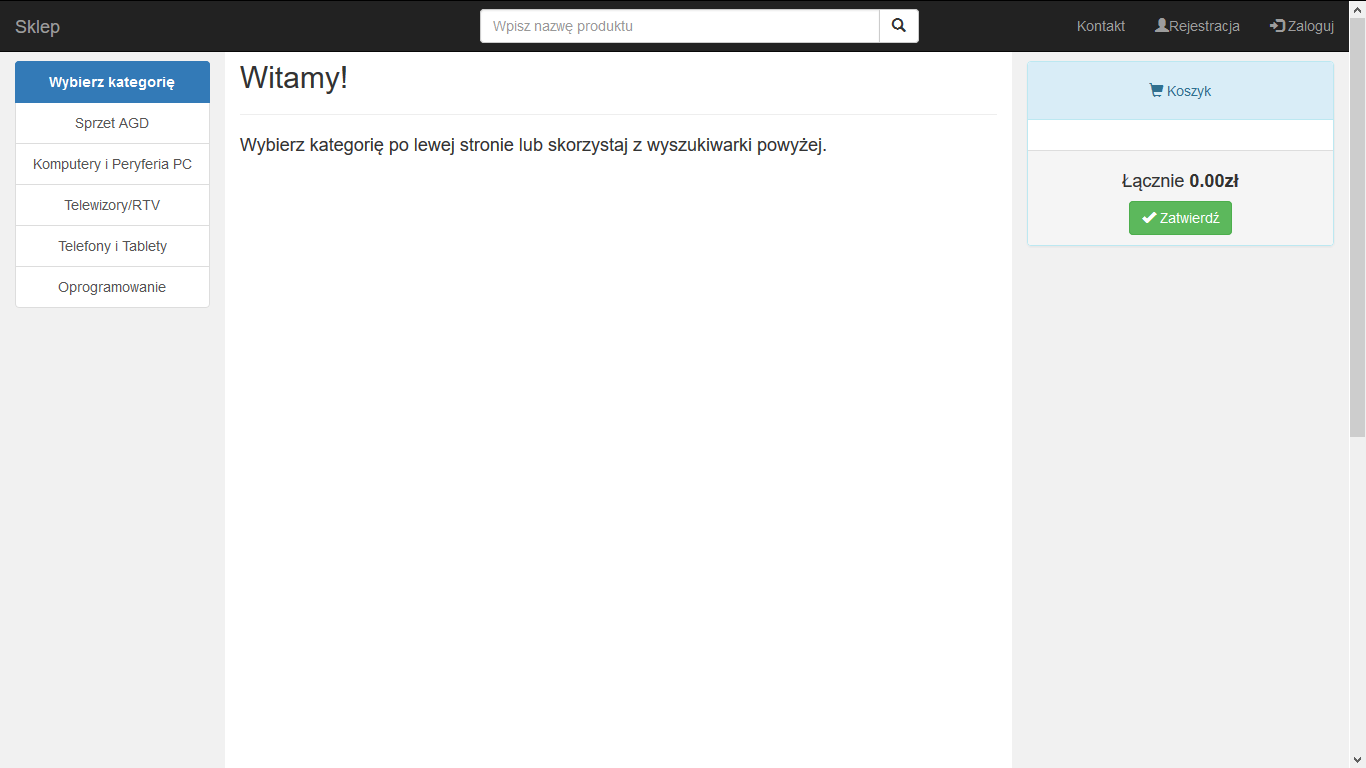
\includegraphics[scale=0.6]{mainpage}
   		\end{figure}
   		
   		\newpage
	    \begin{figure}[H]
   		\caption{Widok Kategorii}
		\centering
   		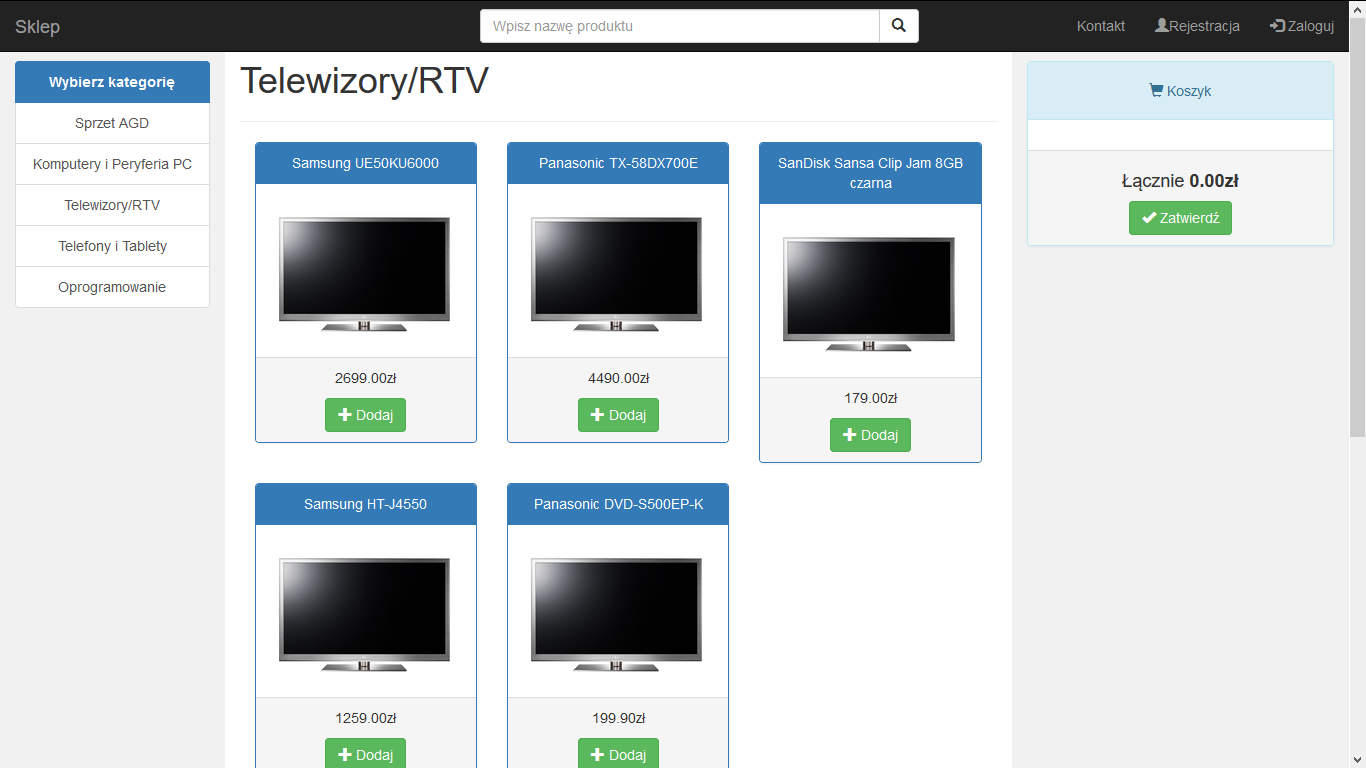
\includegraphics[scale=0.6]{categories}
   		\end{figure}
   		
   		\newpage
   		\begin{figure}[H]
   		\caption{Rejestracja nowego klienta}
   		\centering
   		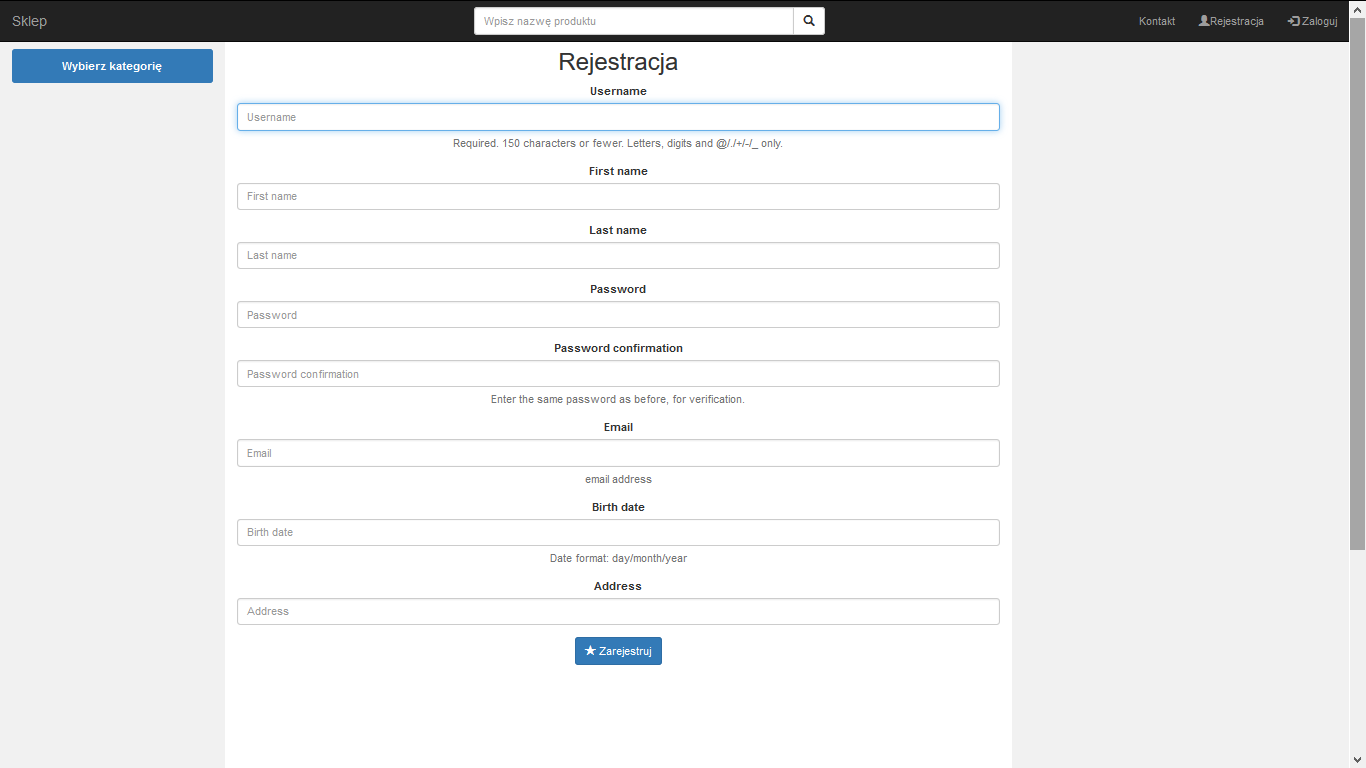
\includegraphics[scale=0.6]{register}
   		\end{figure}
   		
   		\newpage
   		\begin{figure}[H]
   		\caption{Okno logowania}
   		\centering
   		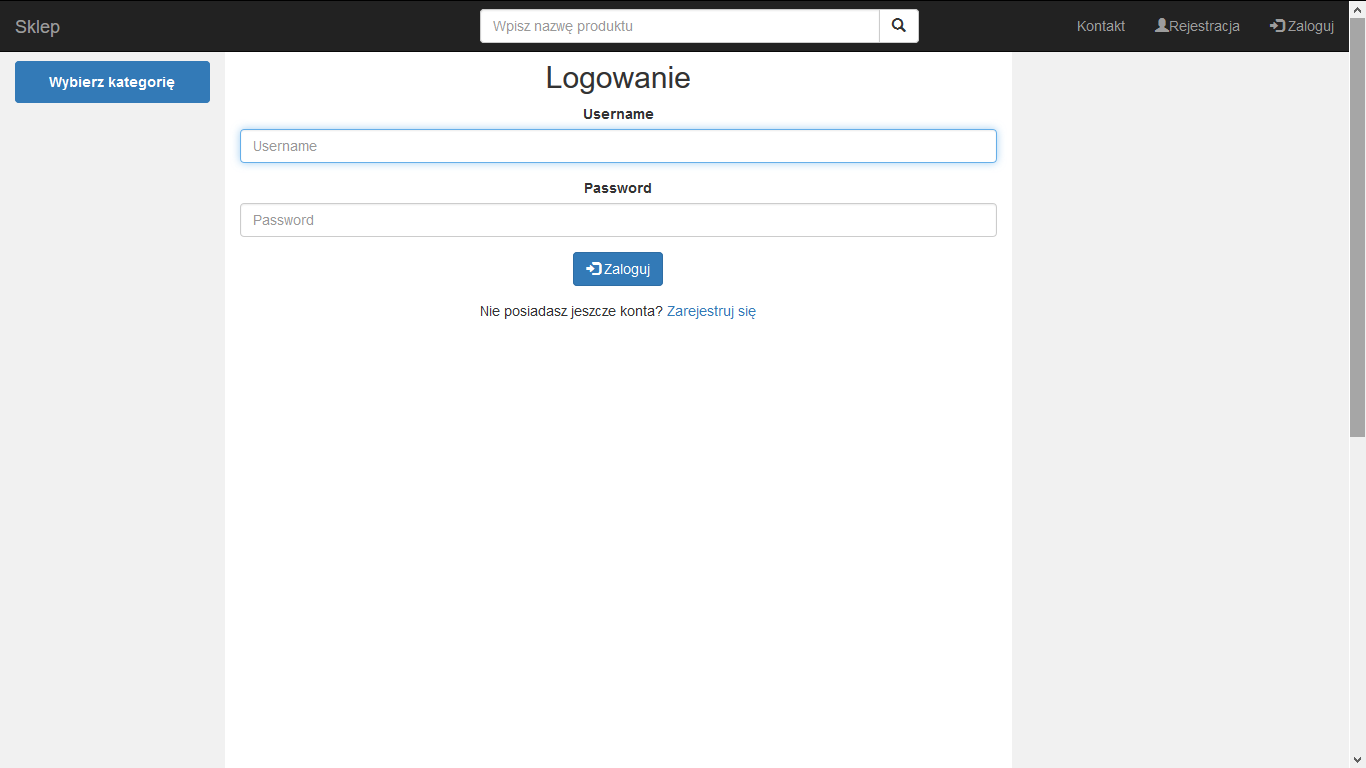
\includegraphics[scale=0.6]{login}
   		\end{figure}
   
   		\newpage
   		\begin{figure}[H]
   		\caption{Zawartość koszyka}
   		\centering
   		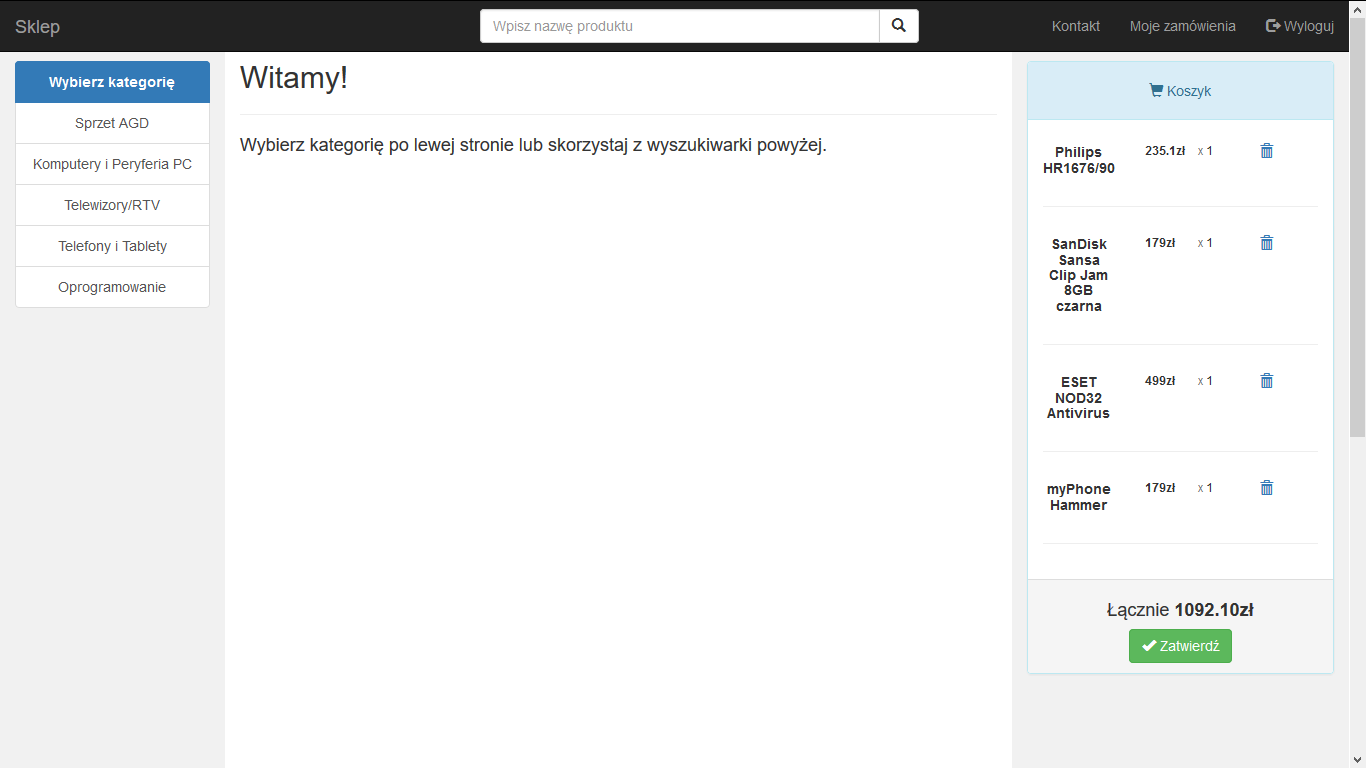
\includegraphics[scale=0.6]{koszyk}
   		\end{figure}
     	
     	\newpage
	    \begin{figure}[H]
   		\caption{Historia zamówień}
   		\centering
   		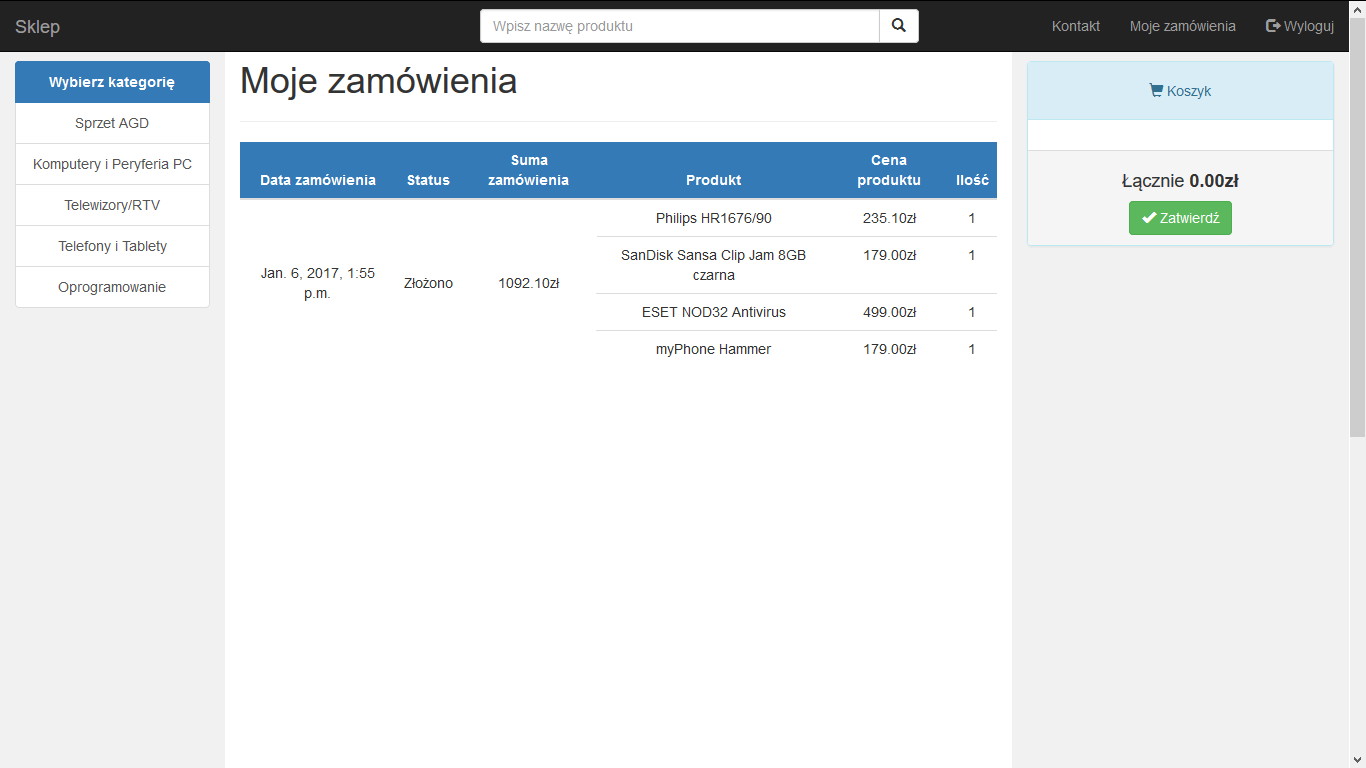
\includegraphics[scale=0.6]{orders}
		\end{figure}
   		
   		\end{landscape}
\end{document}